\documentclass[12pt]{report}
\usepackage[utf8]{inputenc}
\usepackage{amsmath}
\usepackage{amsfonts}
\usepackage{amssymb}
\usepackage[pdftex]{graphicx}
\usepackage{polski}

\usepackage{placeins}
\usepackage{epstopdf}
\usepackage{mathtools}
\usepackage{amsthm}
\usepackage{float}
\usepackage{tabularx}
\usepackage{titlesec}

\titleformat{\chapter}
{\Large\bfseries} % format
{}                % label
{0pt}             % sep
{\huge}           % before-code


\usepackage[left=2.50cm, right=2.50cm, top=2.50cm, bottom=2.50cm]{geometry}

\newcolumntype{C}[1]{>{\hsize=#1\hsize\centering\arraybackslash}X}
\newcolumntype{M}[1]{>{\centering\arraybackslash}m{#1}}

%opening
\title{\textbf{SCADA 2}}
\author{Maciej Cebula \\Piotr Merynda \\Maciej Podsiadło}
\date{}
\begin{document}
	
%	\fancypagestyle{plain}
%	{
%		% Usuń nagłówek i stopkę
%		\fancyhf{}
%		% Usuń linie.
%		\renewcommand{\headrulewidth}{0pt}
%		\renewcommand{\footrulewidth}{0pt}
%	}

	
	\setcounter{tocdepth}{2}
	
	\maketitle
	\tableofcontents
	\clearpage
		
		\renewcommand{\tablename}{Tabela}
		\renewcommand{\figurename}{Rys.}
		
	\chapter{Wstęp}

\section{Opis projektu}



\section{Założenia}


	\chapter{Model Systemu}
\section{System zbiorników}
\indent Przedmiotem rozważań jest system 3 połączonych zbiornkiów. Zbiornik 3 służy jako rezerwuar wody. W zbiorniku 2 znajduje się koncentrat wykorzystywany do produkcji napoju. Oba te zbiorniki umieszczone są nad zbiornikiem 1, w którym woda miesza się z koncentratem tworząc gotowy produkt. Pomiędzy zbiornikami 3 i 1 oraz 2 i 1 znajdują się zawory pozwalające na regulację przepływu cieczy pomiędzy nimi. Poglądowy schemat procesu znajduje się na rysunku \ref{fig:Proces}.
\begin{figure}[H]
	\centering
	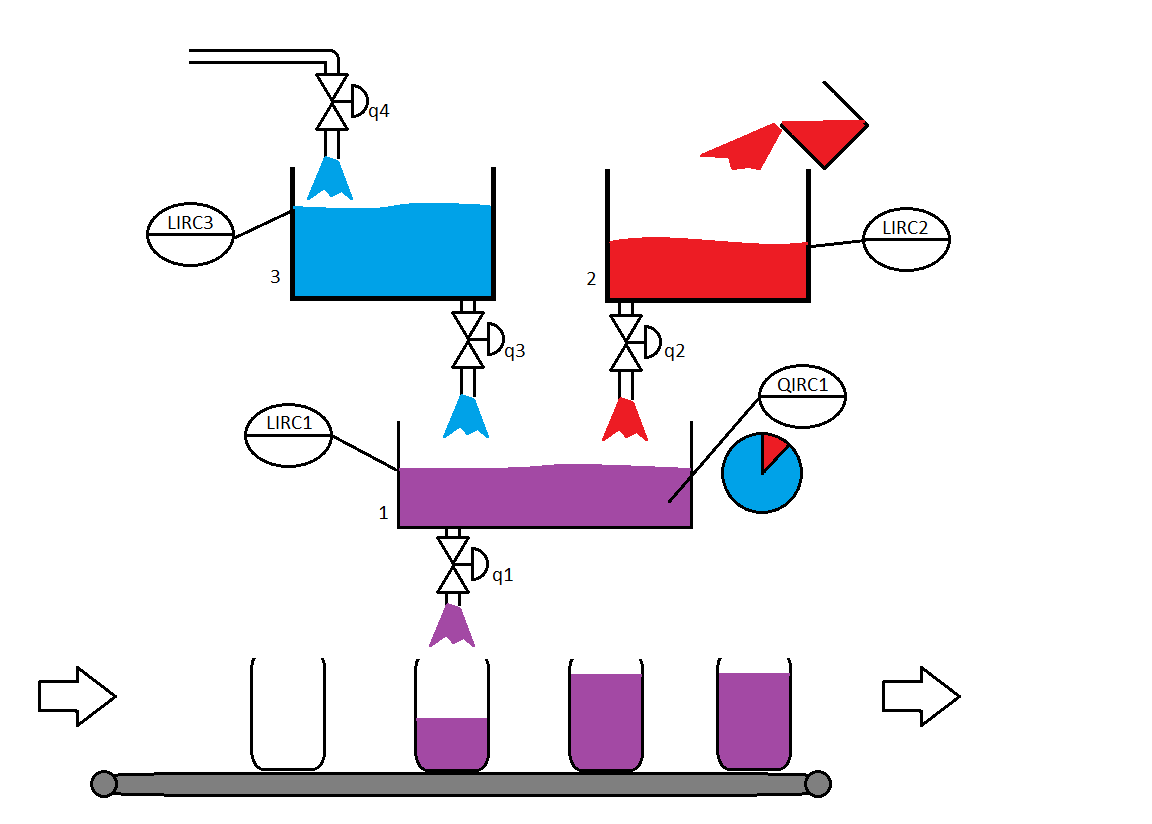
\includegraphics[scale = 0.4]{fig/Proces_schema_updated.png}
	\caption{Schemat procesu.}
	\label{fig:Proces}
\end{figure}

\section{Regulatory}
\subsection{Regulacja poziomu wody w zbiorniku 3}
\indent Regulacja poziomu wody w zbiorniku 3 odbywa się poprzez regulator proporcjonalny sterujący stopniem otwarcia zaworu q4. Wartość sterowania wyliczana jest na podstawie uchybu pomiędzy wartością zadaną {h3\_SV} a wysokością poziomu wody w zbiorniku h3.
\begin{figure}[H]
	\centering
	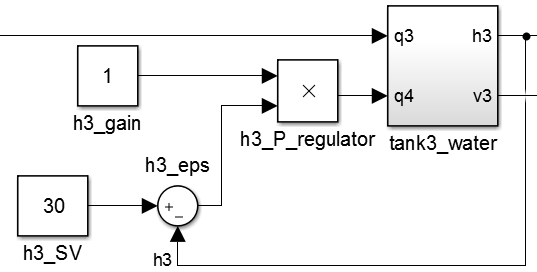
\includegraphics[scale = 0.4]{fig/h3_regulator.png}
	\caption{Schemat regulatora poziomu cieczy h3.}
	\label{fig:h3reg}
\end{figure}
\subsection{Regulacja poziomu koncentratu w zbiorniku 2}
\indent Regulacja poziomu koncentratu w zbiornkiu 2 odbywa się poprzez dolewanie dodatkowych porcji substancji przez pracownika po zgłoszeniu przez system komunikatu o niskim poziomie cieczy w zbiorniku. Aby zamodelować działanie pracownkia, który posiada pewną zwłokę w wykonywaniu działań oraz potrzebuje czasu na przemieszczenie się z dodatkową porcją koncentratu, użyto maszyny stanów. Określono czas reakcji pracowniak na komunikat systemowy, czas potrzebny do zabrania kolejnej porcji, oraz czas potrzebny na uzupełnienie koncentratu.
\subsection{Regulacja dawkowania wody i koncentratu do zbiornika mieszającego}
\indent Regulacja przepływu wody oraz koncentratu do zbiornika mieszającego odbywa się na podstawie pomiaru wysokości cieczy w zbiorniku 1 oraz na podstawie pomiaru stężenia koncentratu w gotowym produkcie. Regulacja odbywa się w taki sposób aby utrzymać zadany poziom w zbiuorniku oraz zadane stężenie gotowego produktu.
\subsection{Regulacja dawkowania gotowej mieszanki ze zbiornika mieszającego}
\indent Regulator odpowiedzialny za napełnianie pojemników gotową mieszanką działa poprzez maksymalne otwarcie wypływu ze zbiornika 1 aż do całkowitego napełnienia się naczynia. Po całkowitym napełnieniu zawór zostaje zamknięty aż do nadejścia kolejnego pojemnika do napełnienia.

	\chapter{Serwer HTTP}
\section{Opis działania}
W celu umożliwienia komunikacji aplikacji wizualizującej z bazą danych napisano w języku \textit{JAVA} serwer HTTP. Dane pomiędzy serwerem i aplikacją wymieniane są za pomocą protokołu HTTP, wykorzystując w tym celu zapytania typu \textit{GET} i \textit{POST}. Wszystkie żądania są utożsamione z odpowiednim adresem url i odpowiednio przetwarzane po stronie serwerowej. Aby zapewnić jak największą responsywność aplikacji oraz synchroniczne odświeżanie danych każdy request po stronie serwera przetwarzany jest w osobnym wątku. \\
Do napisania serwera wykorzystano następujące biblioteki \textit{JAV-wy}:
\begin{enumerate}
	\item \textbf{RXJava} - biblioteka zapewniająca mechanizmy asynchronicznego przetwarzania danych \cite{rxjava},
	\item \textbf{JDBI} - biblioteka zapewniająca połączenie z bazą danych \cite{jdbi},
	\item \textbf{AKKA-HTTP} - framework do implementacji serwera HTTP \cite{akka doc},
	 \item \textbf{Javax mail} - biblioteka do wysyłania emaili.
\end{enumerate}

\section{Uruchomienie serwera}
W momencie pisania sprawozdania w repozytorium \textit{} nie udostępniono jeszcze skompilowanej wersji flików \'zródłowych. Dlatego też w celu uruchomienia aplikacji na komputerze wymagane jest: 
\begin{enumerate}
	\item zainstalowanie Jav-y w wersji 8
	\item zainstalowanie dowolnego środowiska programistycznego \textit{Intellij, Eclipse itp.}
	\item skompilowanie i uruchomienie całego projektu dostępnego pod adresem \\ \textit{https://github.com/maciekc/SCADA2}
\end{enumerate}
	\chapter{Baza danych}

\section{Wstęp}
Aby móc wizualizować przebieg pracy systemu wszystkie najważniejsze dane z punktu widzenia automatyki są logowane w bazie danych. Do tego celu wykorzystano bazę danych typu \textit{MYSQL} i środowisko \textit{MYSQL Workbench}, zainstalowane na jednym z komputerów, którym stworzono całą strukturę przedstawioną na rysunku \ref{fig:db}. Dostęp poszczególnych węzłów systemu do bazy danych zapewniony jest poprzez połączenie wszystkich komputerów w lokalną sieci. 
 

\section{Struktura bazy}

Zaprezentowana na rysunku baza danych na strukturę relacyjną aby zapewnić możliwość ewentualnej rozbudowy sytemu o inne składowe. Z racji na to, że baza służy głównie do logowania pracy systemu podzielono ją na następujące części:
\begin{enumerate}
	\item główną tabele \textbf{history}, w której logowane są wszystkie zdarzenia w kolejności chronologicznej,
	\item tabelę  \textbf{Andon}, w której zapisywane są wszystkie sytuacje alarmowe,
	\item tabelę \textbf{Work}, do której logowany jest stan normalnej pracy systemu,
	\item tabelę \textbf{change\_parameter}, w której zapisywane są wszelkie zmiany wartości parametrów systemu,
	\item tabelę \textbf{controller}, która służy do logowania pracy regulatorów.
\end{enumerate}
%
Dodatkowo:
\begin{enumerate}
	\item w tabeli \textbf{state\_space} zdefiniowano wszystkie zmienne stanu występujące w systemie,
	\item tabele \textbf{variable\_state} definiuje wszystkie możliwe stany danej zmiennej np. Work, Andon, Change parameter itd.
	\item tabela \textbf{limits} definiuje poszczególne limity i przypisuje je do odpowiednich zmiennych stanu z tabeli \textbf{state\_space},
	\item w tabeli \textbf{system\_parameter} zdefiniowane są pozostałe parametry systemu takie jak: nastawy poszczególnych regulatorów, wartości zadane itp.
\end{enumerate}

\newpage
\begin{figure}[H]
	\centering
	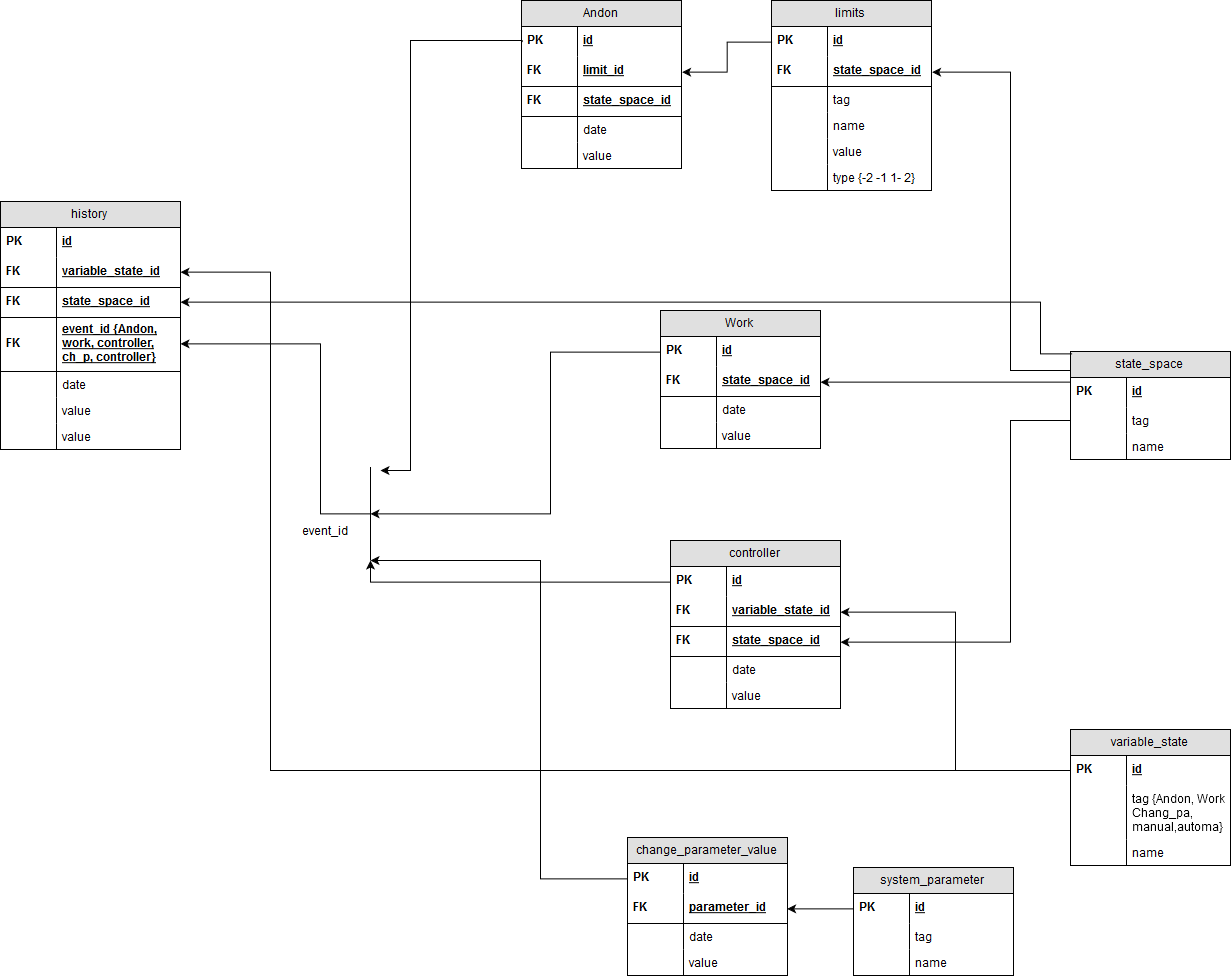
\includegraphics[scale = 0.4]{fig/DB_SCHEMA.png}
	\caption{Struktura bazy danych.}
	\label{fig:db}
\end{figure}

\section{Opis dostępu do bazy}

Dane dotyczące parametrów systemu w poszczególnych chwilach czasu są logowane przez serwer OPC i następnie prezentowane w aplikacji.  
	\section{Serwer OPC}
\subsection{Wprowadzenie}
Systemy typu PLC – SCADA są powszechnie wdrażane poczynając od przemysłu chemicznego, a kończąc na automatyce budynków. Stanowią pewną normę w nowoczesnych zakładach oraz fabrykach. W związku z bogatą ofertą producentów aparatury automatyzacji powstał problem komunikacji pomiędzy różnymi komponentami. Firmy promowały swoje rodzime protokoły przemysłowe, co wymuszało na końcowych użytkownikach stosowanie sprzętu pochodzącego od tego samego producenta w obrębie całego obiektu. Przełomem okazało się wprowadzenie otwartego rozwiązania – standardu OPC. OPC jest standardem umożliwiającym komunikację pomiędzy sterownikami (najczęściej PLC) a oprogramowaniem SCADA. Bazuje na modelu klient-serwer, przy czym strona serwera zaimplementowana jest w oprogramowaniu dostarczanym przez producentów sterowników, natomiast klientem - aplikacja wykorzystująca udostępniane dane. 
\subsection{MatrikonOPC}
Dla celów zintegrowania omawianego systemu zastosowano testowy serwer udostępniony przez firmę Matrikon służący do celów niekomercyjnych. Dostawca oferuje serwer OPC (OPC Simulation Server), jak również oprogramowanie do zarządzania odczytywanymi danymi (OPC Explorer). 
%TODO konfiguracja serwera
\subsection{Logowanie OPC - MySQL}
Kolejny element stworzonego wielopoziomowego systemu sterowania stanowi aplikacja logująca aktualne dane pochodzące z serwera OPC do procesowej bazy danych. Aplikacja napisana została w języku C\#. Do komunikacji z serwerem użyto open sourcową bibliotekę TitaniumAS.Opc (https://github.com/titanium-as/TitaniumAS.Opc.Client). Serwer lokalizowany jest jedynie po nazwie, co, zgodnie z ideą OPC, znacząco przyspiesza proces integracji. Aplikacja odczytuje bieżące pomiary z serwera OPC z zadaną przez użytkownika częstotliwością, a następnie loguje je w bazie danych MySQL. Podstawową częstotliwością odpytywania jest 1 sekunda, tak jak to ma miejsce w większości systemów typu SCADA. Poszczególne pomiary identyfikowane są po tagach jakie zostały im nadane w momencie inicjalizacji w serwerze OPC. Zapis do bazy danych odbywa się według konwencji narzuconej w momencie jej zaprojektowania. Aplikacja zapewnia mechanizmy przechwytywania zgłaszanych błędów, w szczególności błędów połączenia z serwerem oraz MySQL. Użytkownik informowany jest o napotkanym błędzie. Program dokonuje niezbędnej konwersji sposobu zapisu liczb zmiennoprzecinkowych, zamienia separator ‘,’ na ‘.’ bez czego zapis do bazy danych nie byłby możliwy.
 
Warto nadmienić, że użytkownik operujący na systemie Windows nie musi instalować, żadnego dodatkowego oprogramowania w celu uruchomienia omawianej aplikacji logującej.

	\chapter{Aplikacja}
\section{Opis działania aplikacji}
Głównym założeniem aplikacji wizualizującej pracę systemu było zaprezentowanie pracy sytemu w sposób przejrzysty i uporządkowany. Dodatkowo aplikacja powinna umożliwiać zmianę wybranych parametrów systemy oraz zapewniać jednoczesny dostęp dla wielu użytkowników. Biorąc pod uwagę wymienione wymagania zdecydowano się na napisanie aplikacji webowej wykorzystując do tego celu framework \textit{Angular 4 - https://angular.io/}.
\section{Opis okien}
Aplikacja do wizualizacji pracy systemu podzielona jest na 5 ekranów. 
\begin{enumerate}
	\item \textbf{Schemat} - przedstawia schemat rozpatrywanej instalacji,
	\item \textbf{Statystyki} - przedstawia najważniejsze dane opisujące aktualny stan instalacji takie jak: poziomu cieczy w każdym ze zbiorników, aktualne stężenie, a także przebiegi czasowe tych sygnałów zaprezentowane za pomocą wykresów,
	\item \textbf{Obiekt} - prezentuje szczegółowe dane dotyczące obiektu regulacji oraz daje możliwość zmieniania limitów w każdym ze zbiorników.
	\item \textbf{Regulator} - przedstawia przebiegi czasowe sygnałów sterowania, a także daje możliwość zmieniania nastaw regulatorów,
	\item \textbf{Logi} - daje możliwość generowania raportów z wybranych stanów pracy systemu tzn: zwykła praca, stany alarmowe, zmiany wartości parametrów systemu.
\end{enumerate}
Każdy z ekranów na składa się z trzech głównych części \ref{fig:sc0}:
\begin{enumerate}
	\item Pasek menu - umożliwia przechodzenie pomiędzy wszystkimi oknami aplikacji,
	\item \textbf{Panel danych} - w jego obszarze wyświetlane są dane dotyczące poszczególnych funkcjonalności systemu,
	\item \textbf{Pasek wiadomości} - Wyświetlane są na nim najważniejsze wiadomości dotyczące pracy systemu takie jak np. przekroczenie limitów.
\end{enumerate}

\section{Alarmy}
Każdy zbiornik ma zdefiniowany zestaw czterech limitów poziomu cieczy tzn. 
\begin{enumerate}
	\item Limit minimalny krytyczny,
	\item Limit minimalny,
	\item Limit maksymalny,
	\item Limit maksymalny krytyczny
\end{enumerate}
Wartości wyżej wymienionych limitów mogą być monitorowane oraz zmieniane przy wykorzystaniu ekranu \textit{Obiekty}. Każda zmiana wartości jest automatycznie zapisywana w bazie danych i propagowana do regulatora.

W aplikacji zaimplementowano również propagację alarmów. W momencie przekroczenia dowolnego ze zdefiniowanych limitów pod wskazany adres wysyłany jest email informujący o tym zdarzeniu. 

\section{Regulatory}
Aplikacja daje możliwość operatorowi na zdalną zmianę parametrów regulatorów za pomocą ekranu \textit{Regulator}. Podobnie jak w przypadku alarmów każdorazowa zmiana dowolnego parametru jest propagowana do regulatora i zapisywana w bazie danych.
\section{Wygląd aplikacji}
Na poniższych rysunkach przedstawiono screen-y z działania opisywanej aplikacji dla każdego z dostępnych ekranów.
\begin{figure}[H]
	\centering
	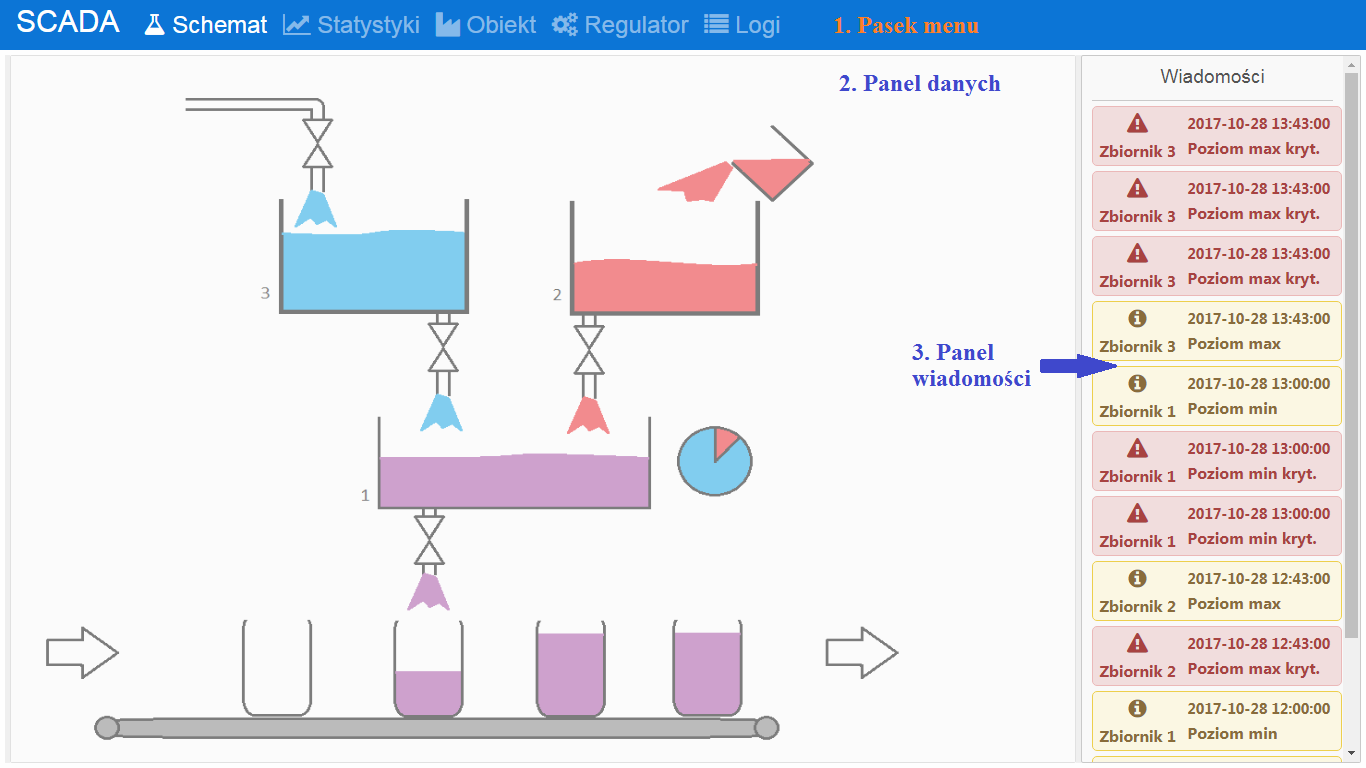
\includegraphics[scale = 0.45]{fig/sc0.png}
	\caption{Budowa ekranu.}
	\label{fig:sc0}
\end{figure}


\begin{figure}[H]
	\centering
	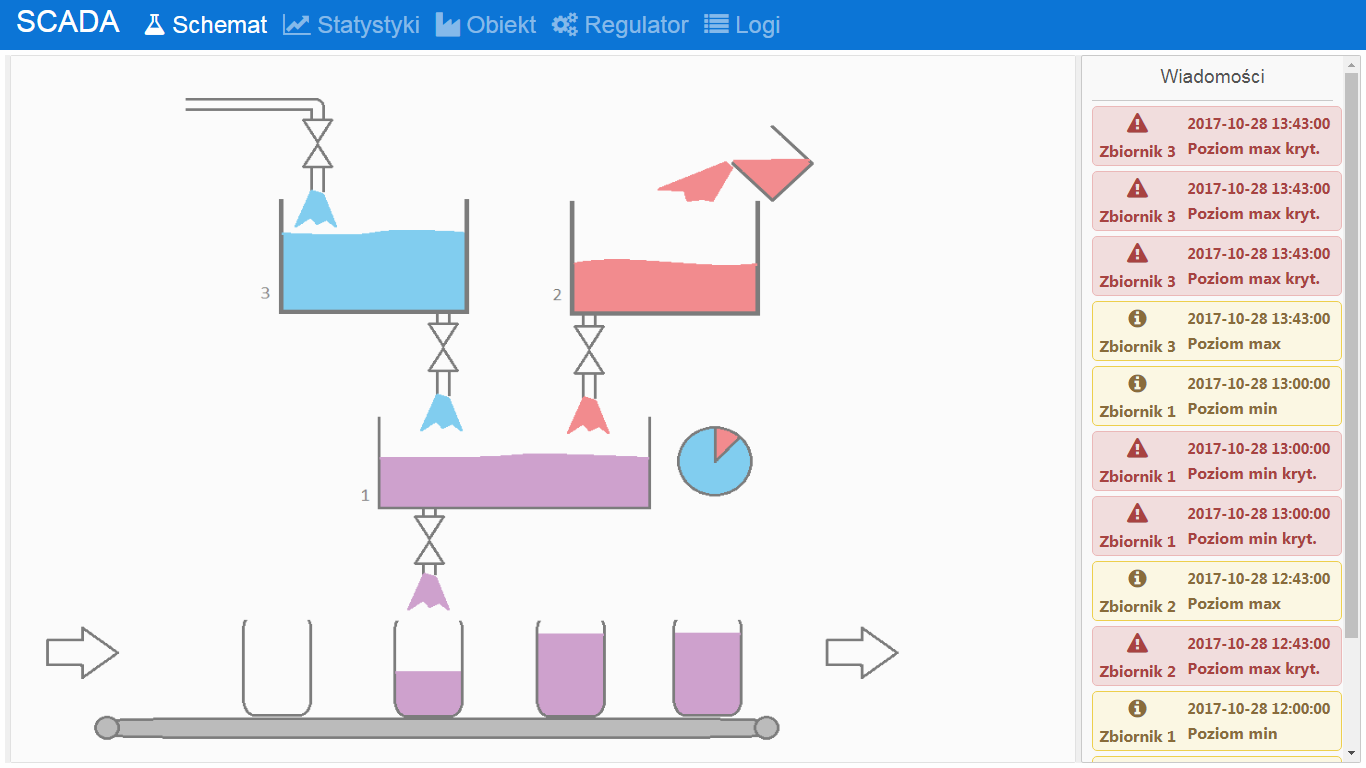
\includegraphics[scale = 0.45]{fig/sc1.png}
	\caption{Schemat systemu.}
	\label{fig:sc1}
\end{figure}

\begin{figure}[H]
	\centering
	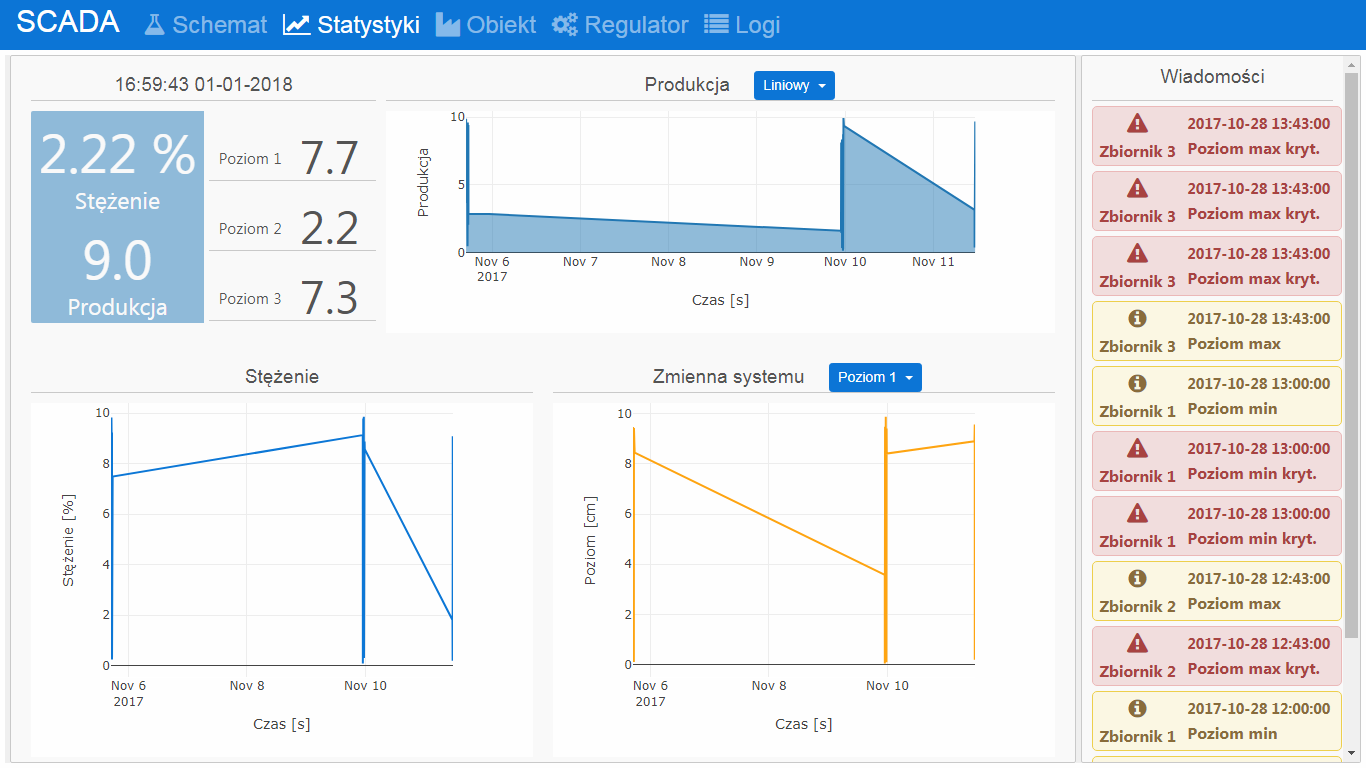
\includegraphics[scale = 0.45]{fig/sc2.png}
	\caption{Statystyki systemu.}
	\label{fig:sc2}
\end{figure}

\begin{figure}[H]
	\centering
	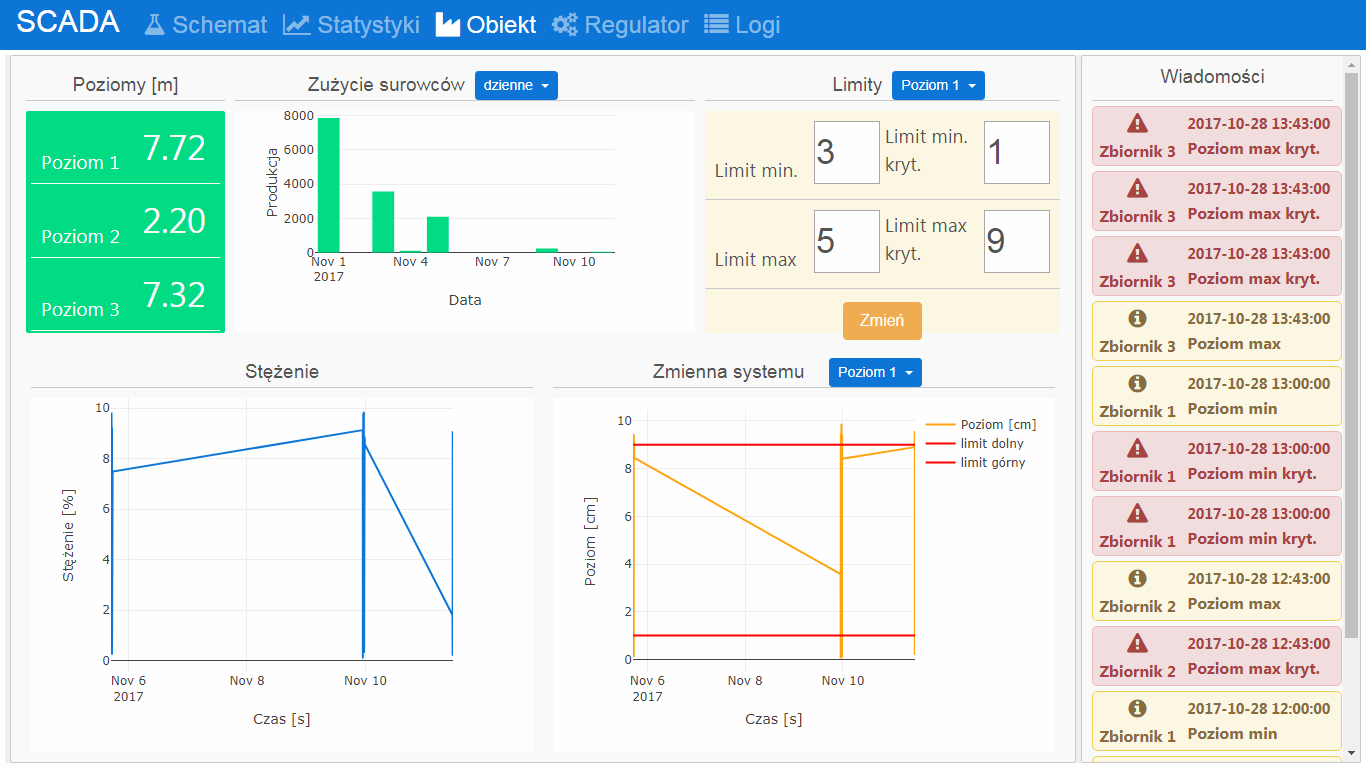
\includegraphics[scale = 0.5]{fig/sc3.png}
	\caption{Ekran przedstawiający stan instalacji.}
	\label{fig:sc3}
\end{figure}

\begin{figure}[H]
	\centering
	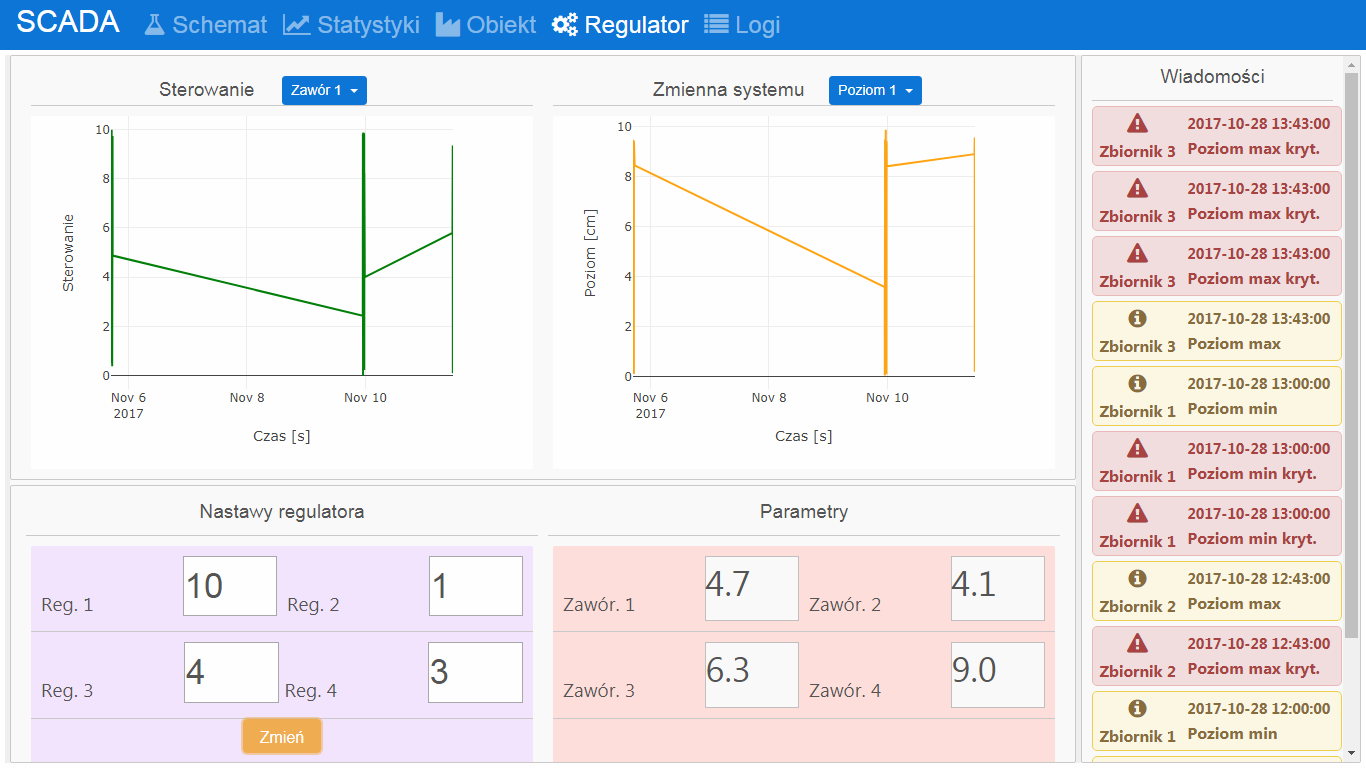
\includegraphics[scale = 0.5]{fig/sc4.png}
	\caption{Ekran przestawiający pracę regulatorów.}
	\label{fig:sc4}
\end{figure}

\begin{figure}[H]
	\centering
	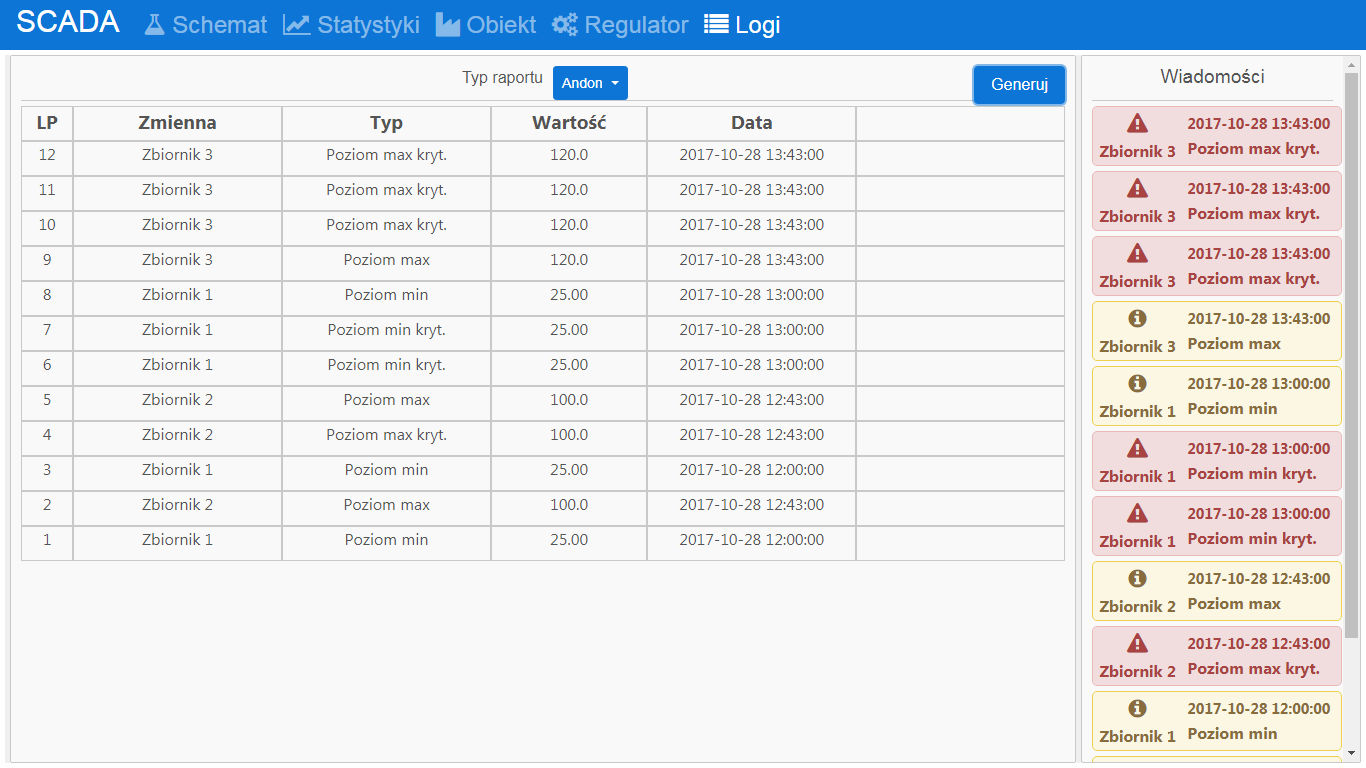
\includegraphics[scale = 0.5]{fig/sc5.png}
	\caption{Ekran do generowania raportów.}
	\label{fig:sc5}
\end{figure}

\section{Uruchomienie aplikacji}
Do uruchomienie aplikacji należy: 
\begin{enumerate}
	\item na wybranym komputerze zainstalować serwer \textit{Node.js - https://nodejs.org/en/}
	\item  pobrać kod \'zródłowy projektu ze strony \textit{https://github.com/maciekc/SCADA2}
	\item w konsoli systemu \textit{Windows} należy przejść do głównego folderu projektu  \textit{SCADA-app} i wywołać procedurę \textbf{npm start}
	\item od tej pory aplikacja będzie dostępna pod adresem \textit{www.localhost:4200}.
	
\end{enumerate}
	\begin{thebibliography}{}
	
	%przykład 
	
%	\bibitem{pauluk 1}Pauluk, M.: 
%	\emph{Model matematyczny trójwymiarowej suwnicy.} W: \textbf{Automatyka} 2002 tom 6 s. 69-102, ISSN: 1429-3447
%	

	
\end{thebibliography}
	
\end{document}